\twocolumn[{%
\makeatletter
\section{Interaction Trace and Test Cases}\label{app:trace}\label{app:tests}
\centering
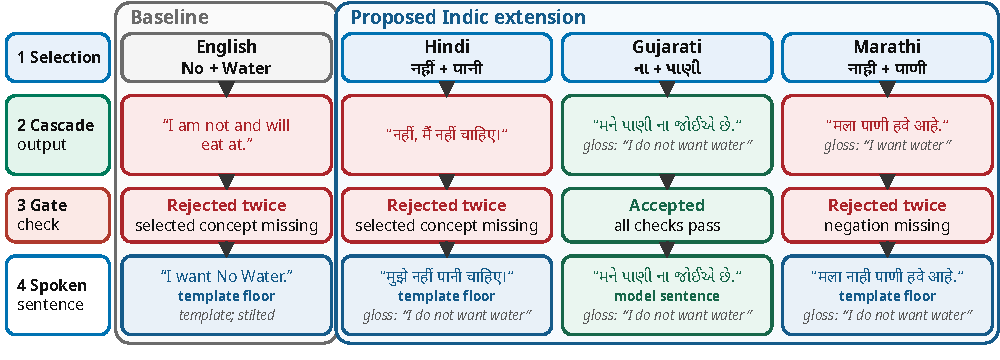
\includegraphics[width=\textwidth]{figures/fig4_languages.pdf}
\captionof{figure}{One selection (\emph{No}\,+\,\emph{Water}) in four languages (recorded outputs). English is the baseline language; Hindi, Gujarati, and Marathi are the proposed extension. Red: rejected cascade output; blue: template floor; green: accepted model sentence; italics: the authors' English gloss. The word order of the template sentences is not native-reviewed.}
\label{fig:workflow}
\vspace{2pt}
\centering\footnotesize
\setlength{\tabcolsep}{3.2pt}\renewcommand{\arraystretch}{1.1}
\begin{tabular}{@{}L{2.5cm}L{2.95cm}L{2.85cm}L{3.0cm}L{3.0cm}@{}}
\toprule
\rowcolor{headtint}
Family: selection & \lang{English} (baseline) & \lang{Hindi} & \lang{Gujarati} & \lang{Marathi} \\
\midrule
Request: \emph{Fruit}
 & \kept{I want Fruit.} \routet\ \okmark
 & \hi{\kept{मुझे फल चाहिए।}} \routem\ \okmark
 & \gu{\kept{મને ફળ જોઈએ છે.}} \routem\ \okmark
 & \hi{\kept{मला फळ हवे आहे.}} \routem\ \okmark \\
\rowcolor{rowtint}
Refusal: \emph{No}\,+\,\emph{Fruit}
 & \bad{I am not a} \sel{fruit}\bad{. I do not eat fruits.} \routem\ \failmark{W,A}
 & \hi{\kept{फल नहीं है, नहीं चाहिए।}} \routem\ \okmark
 & \gu{\sel{મારે ના ફળ છે.}} \routem\ \failmark{N}
 & \hi{\kept{मला नाही फळ हवे आहे.}} \routet\ \okmark \\
Feeling: \emph{Angry}
 & \bad{I want} \sel{Angry.} \routet\ \failmark{W}
 & \hi{\bad{मुझे} \sel{गुस्सा} \bad{चाहिए।}} \routem\ \failmark{W}
 & \gu{\bad{મને} \sel{ગુસ્સો} \bad{જોઈએ છે.}} \routem\ \failmark{W}
 & \hi{\bad{मला} \sel{रागात} \bad{हवे आहे.}} \routem\ \failmark{W} \\
\rowcolor{rowtint}
Negated feeling: \emph{No}\,+\,\emph{Angry}
 & \bad{I want} \sel{No Angry.} \routet\ \failmark{W}
 & \hi{\sel{गुस्सा,} \bad{नहीं चाहिए।}} \routem\ \failmark{W}
 & \gu{\sel{મારે ના ગુસ્સો છે.}} \routem\ \failmark{N}
 & \hi{\bad{मला} \sel{नाही रागात} \bad{हवे आहे.}} \routet\ \failmark{W} \\
Action: \emph{Drink}\,+\,\emph{Milk}
 & \bad{The user requested} \sel{milk} \bad{for their drink.} \routem\ \failmark{N,P}
 & \hi{\kept{मुझे पीना दूध चाहिए।}} \routet\ \okmark
 & \gu{\kept{મને પીવું જોઈએ છે. દૂધ આપે.}} \routem\ \okmark
 & \hi{\kept{मला पिणे दूध हवे आहे.}} \routem\ \okmark \\
\rowcolor{rowtint}
Call: \emph{Call}\,+\,\emph{Doctor}
 & \kept{I want Call Doctor.} \routet\ \okmark
 & \hi{\kept{फ़ोन करना गया है, मुझे डॉक्टर चाहिए।}} \routem\ \okmark
 & \gu{\sel{મને ડૉક્ટર ફોન કરવો છે.}} \routem\ \failmark{N}
 & \hi{\sel{मला डॉक्टर फोन करणे मिळू शकता का?}} \routem\ \failmark{N} \\
\bottomrule
\end{tabular}
\captionof{table}{One scenario per family (the first in alphabetical order that is in the primary set for all four languages), deployed output with web-client input (recorded). Intended messages: \gloss{I want fruit}, \gloss{I do not want fruit}, \gloss{I am angry}, \gloss{I am not angry}, \gloss{I want to drink milk}, \gloss{I want to call the doctor}. Colors, marks, and tags as in Table~\ref{tab:analysis}; \failmark{P} is a third-person report. No native speaker has judged these outcomes; the Gujarati and Marathi \emph{Call} outputs are a scorer gap and a question form.}
\label{tab:grid}
\makeatother
}]

\begin{table*}[t]
\centering\footnotesize
\setlength{\tabcolsep}{3.2pt}\renewcommand{\arraystretch}{1.1}
\begin{tabular}{@{}L{2.6cm}L{3.0cm}L{6.2cm}L{3.2cm}@{}}
\toprule
\rowcolor{headtint}
Kind of outcome & Input & Recorded output & Result \\
\midrule
Concept replaced, caught & \lang{English}, client: \emph{Water} & cascade \bad{I need food.}; spoken \sel{I want Water.} \routet & rejected twice (selected concept missing) \\
\rowcolor{rowtint}Polarity inverted, caught & \lang{Marathi}, explicit: \emph{No}\,+\,\emph{Water} & cascade \hi{\bad{मला पाणी हवे आहे.}} (\gloss{I want water}); spoken \hi{\sel{मला पाणी नको आहे.}} \routet & rejected (negation missing); template \\
Accepted, third person & \lang{English}, client: \emph{Tired} & \bad{The user is tired of waiting for their meal and wants to go out to eat.} \routem & accepted by the gate; fails scorer (added content, third person) \\
\rowcolor{rowtint}Ambiguous selection; server unreachable (repaired client) & \lang{English}: \emph{Nose}; any language & card \gloss{What do you want to say?} with buttons \gloss{I want something} and \gloss{I feel something}; the literal labels, marked as a preview & nothing is spoken until the user chooses; nothing is guessed \\
\bottomrule
\end{tabular}
\caption{One recorded example of each further kind of outcome (colors and tags as in Table~\ref{tab:analysis}); the Gujarati scorer gap is in Section~\ref{sec:eval}. The last row shows demo states captured from the repaired build, not scored scenarios.}
\label{tab:kinds}
\end{table*}


\begin{table*}[t]
\centering\footnotesize
\setlength{\tabcolsep}{3pt}\renewcommand{\arraystretch}{1.08}
\begin{tabular}{@{}L{2.9cm}L{2.4cm}L{7.6cm}L{2.5cm}@{}}
\toprule
\rowcolor{headtint}
Component & Role in the demo & Training or adaptation & Data \\
\midrule
\qwen{} (rev.\ 7ae5576) & realizer, refiner, verifier & Prompted, not fine-tuned (few-shot for HI, GU, MR) & -- \\
\indicf{} + \vocos{} & speech & Pretrained; zero-shot voice conditioning on a clip and its transcript & 1,417\,h, four corpora \\
HMM-1, HMM-2 & optional next word; Un-Jumble & Streamed in 500K-sentence chunks, count-pruned; HMM-1: Jelinek--Mercer weights .50/.30/.15/.05; HMM-2: word and POS trigrams, beam 64 & English sentences, Tatoeba, Pile slices \\
Gutenberg HMM; Hindi AAC HMM & English baseline; Hindi fallback & Bigram and trigram counts over 188,402 sentences (713,845 trigram states); 3,867 Hindi turns, 2,171 word types (3,078 turns for evaluation) & public-domain books; Hindi dialogues \\
Suffix trie ($\infty$-gram) & primary next word & Count-based, built at start-up (\IGSent{} sentences, depth \IGDepth{}) & EN and HI dialogues \\
\flant{} refiner & companion tool & Fine-tuned: learning rate $10^{-4}$, batch 16 with two accumulation steps, 10 epochs, seed 42, one TITAN Xp (204\,s); 500-update fluency adaptation on 4,380 denoising pairs & 3,052 template payloads (384 validation, 384 test) \\
\bottomrule
\end{tabular}
\caption{Learned components, from the training records, run configurations, and model files in the release package; \qwen{} and \indicf{} are used as released. The \indicf{} corpora are Rasa, IndicTTS, LIMMITS, and IndicVoices-R. Licenses: \qwen{} Apache-2.0, \vocos{} MIT, \indicf{} MIT (gated download), Noto fonts SIL OFL 1.1. On its 384 test payloads the refiner reaches \RefAModel{} exact match (\RefFModel{} with the adaptation) and no negation error in 172 negated payloads, at a median of \RefALat{}\,ms; rules and the hybrid score \RefARules{} because the references come from the same template families.}
\label{tab:models}
\end{table*}

\section{Scorer Definitions and Failure Audit}
\label{app:scorer}
Retention is the share of required concept instances present (lexicon forms with inflection stems). Polarity is correct when a negator is present exactly if the gold message is negated, and the act is correct when a request marker (want, need, \hi{चाहिए}, \gu{જોઈએ}, \hi{हवे}) or, for feelings, a feeling marker without a request marker is present. A concept is \emph{added} if any other board concept or a time, meal, or venue word occurs.
An output is \emph{off-task} if it is a model refusal or meta-comment, a third-person report (``the user\ldots''), empty, longer than 25 tokens, or contains Latin text in an Indic target; a user's own refusal (\gloss{I do not want water}) is never off-task.
\emph{Failure audit.} Of the 37 accepted outputs that fail the scorer with explicit fields, 35 are genuine failures (12 negated want for a negated feeling, 10 ungrammatical, 9 third-person reports, 4 added content) and two are marker-list gaps, as are all six failing template fallbacks and all eight failing template-only outputs (the authors' classification, not native-checked).

\begin{table}[t]
\centering\footnotesize
\setlength{\tabcolsep}{2.6pt}
\begin{tabular}{@{}lcccccc@{}}
\toprule
 & \multicolumn{3}{c}{Client payload} & \multicolumn{3}{c}{Explicit fields} \\
\cmidrule(lr){2-4}\cmidrule(l){5-7}
Scenario family ($n$) & Pre & Dep. & Tmpl & Pre & Dep. & Tmpl \\
\midrule
Food/drink request (35) & 26 & 29 & 35 & 26 & 29 & 35 \\
Refusal (\emph{No}+food) (38) & 19 & 33 & 38 & 10 & 38 & 38 \\
Feeling (30) & 3 & 4 & 5 & 18 & 22 & 30 \\
Negated feeling (32) & 2 & 1 & 0 & 2 & 13 & 24 \\
Action + object (24) & 8 & 18 & 24 & 8 & 18 & 24 \\
Help/call + person (16) & 7 & 12 & 16 & 7 & 12 & 16 \\
\midrule
All (175) & 65 & 97 & 118 & 71 & 132 & 167 \\
\bottomrule
\end{tabular}
\caption{Successful scenarios by family on the primary set. Pre: cascade before the gate; Dep.: deployed output; Tmpl: template floor. Exploratory Hinglish ($n=8$; client, explicit): deployed \CMSuccDepU{}, \CMSuccDepS{}; unconstrained prompt \CMSuccNaive{}; template \CMSuccTmplU{}, \CMSuccTmplS{}.}
\label{tab:type}
\end{table}


\section{Language Coverage and Runtime}
\label{app:coverage}
Text generation and next-word coverage are described in Section~\ref{sec:system}. Speech goes to \indicf{} (English is not on its model card), with browser fallback voices hi-IN, gu-IN, and mr-IN (Gujarati and Marathi fall back to hi-IN, then en-IN) and en-US, en-IN, or en-GB; it was not verified in any language because the gated weights were absent and the test browser exposed no voices.
Gate-accepted requests took a median of \LatMedAccEN{}, \LatMedAccHI{}, \LatMedAccGU{}, and \LatMedAccMR{}\,s (EN, HI, GU, MR) and twice-rejected ones \LatFbMin{}--\LatFbMax{}\,s on the GTX~1650 (text generation only); on the repaired build, click to first playback of the placeholder tone had a median of 9.9\,s (95th percentile 20.8\,s; 31 warm runs), so time to audible speech is unmeasured.
In a fresh CPU environment the documented request took 44\,s (the weight download and a GPU installation were not tested); with downloads disabled and non-local connections refused, generation and prediction completed, the only outbound attempt being an optional service.

